\documentclass[11pt]{artikel3}
\usepackage{fullpage, setspace, graphicx}
\usepackage[margin=1in]{geometry}
\usepackage{times}
\usepackage{graphicx}
\usepackage{amsmath}
\usepackage[table]{xcolor}

\title{RIT Department of Computer Science\\MSc Project/Thesis Pre-Proposal:\\\emph{Substructure and Semantic Similarity Search for Documents
Containing Math Formulas}}
\author{Student: Wei Zhong, Advisor: Richard Zanibbi}
\date{\today}

\begin{document}
\maketitle

\textbf{Alternative title:} Combining structural search with fulltext search for documents containing mathematical formulas.

\section{Thesis Statement / Hypothesis}
A math-aware search model using learning-to-rank is able to produce effective results while still being efficient. 
Those features include: Common tree matching based scoring for math formula with IDF weights, TF-IDF and proximity scoring for text terms, embedding generated for math formulas and query expansion suggested from language-topic models.

More specific hypotheses include:
\begin{enumerate}
	\item Multi-subtree matching on formula representation in OPT can produce high relevance search results.~\cite{zhong2019structural}
	\item A single subtree matching model that incorporates dynamic pruning and initial threshold is able to achieve state-of-the-art efficiency, while still maintaining highly relevance results.~\cite{zhong2020speed}

	\item With IDF incorporated into structure matching scoring function, we can obtain better search results for formulas.
	\item Visual Embedding generated by language model and image-to-markup translation model is a good representation for partial formula similarity. Because the inputs are visual image for formulas, and if the model can translate visual features to markups, we assume its hidden states may contain good embedding for visual representation of formulas.
	\item Topic-language model can be used to generate effective global knowledge about document where simple summation of scores from individual keywords do not yield good search results.
	\item Math-aware search can be more effective by assembling above methods and combine scores from different modal linearly using learning to rank.
\end{enumerate}

\section{Contributions}
\begin{itemize}
\item An effective and consistent structural formula retrieval model using multi-tree matching.
\item An efficient structural formula retrieval model for highly relevant results.
\item Introducing IDF into structure formula search that improves retrieval effectiveness.
\item A virtual two-level index to build conceptual unified inverted index for classical fulltext search and structural math search. Because in path-based inverted index, the entries contains docID and expID. To consistently merge with normal text entries which use docID, we need to build an additional layer of "virtual" posing list which hides the merge logics of expID.
\item Combining suitable topic model and formula embedding to boost overall search performance and address the weakness of structure based retrieval approach (e.g., low partial relevance and few global similarity information).
\end{itemize}

\section{Related work}

\subsection{Text-based formula retrieval}
\begin{itemize}
\item DLMF from NIST~\cite{miller2003technical, youssef2005search}: Serialized TeX-favor query language, search them using text search and TF-IDF. 
\item MIaS~\cite{sojka2011indexing, sojka2011art}: Extracting compact strings from  Canonical MathML representation (reordered in alphabetical order). Indexing subexpressions from all depth levels. Searched by Lucene.
\item Kumar et al. from India~\cite{kumar2012structure}: Longest common sub-sequence algorithm performed on augmented preprocessed LaTeX strings, considering matching height in scoring.
\item Kai Ma et al. from Singapore~\cite{ma2010feature}: Feature extractions (semantic MathML, structure feature, number and variables). Clustering features using K-mean on feature TF-IDF. And search query only in its belonged cluster.
\end{itemize}


\subsection{Tree-based formula retrieval}
\begin{itemize}
\item Cyril Laitang et al. from France~\cite{laitang2011xml}: TF-IDF for leaf nodes, and recursively compute score using tree edit distance. To cope with computation complexity, it adopts Dalamagas summary rules to reduce index size.
\item Kamali and Tompa: \cite{kamali2010new} Extract subtrees from normalized Presentation MathML tree, create a DAG index which only indexes one each subtree once and allow subexpressions to point to them. Perform Boolean retrieval on DAG in a recursive fashion. Later in \cite{kamali2013structural}, they choose to use tree edit distance to calculate a similarity score. To compensate efficiency, they do early termination and subexpression caching.
\item WikiMirs from Peking~\cite{hu2013wikimirs}: extract substructures (exact and generalized) from a self-defined presentation tree. Perform exact linearised substructure match and rank them by TF-IDF.
\item Whelp~\cite{asperti2004content} from Italy: Apply automatic theorem proving tools, i.e. Coq, to match a set of indexed expressions having the same computed output. Results are joined in a database.
\item MathWebSearch~\cite{kohlhase2006search,kohlhase2008mathwebsearch,kohlhase2012mathwebsearch}: Term index technique, perform query on tree index with sub-trees augmented.
\item Tangent-S: SLT/OPT tuple pairs with re-ranking stage to find maximum matched tree measured by common nodes and edges.
\item Tangent-CFT: Apply fastText Embedding to formulas SLT/OPT compact strings, sum vectors with operator types embedding.

\item \textbf{Systems/papers using similar approaches as ours:}
\item Hiroya Hagino and Hiroaki Saito~\cite{hagino2013partial} uses leaf-root paths from each node to root. We use the reverse direction, and we perform structure common tree matching.
\item Yoshinori Hijikata, Hideki Hashimoto and Shogo Nishida~\cite{hijikata2007investigation, hijikata2009search} uses exact XPath match (complete leaf-root path) and leaf node symbol. We also use prefix of leaf-root paths, in query as well as in index. Also, they only use ``first" and deepest path to represent a formula.
\item Yokoi, Keisuke and Aizawa, Akiko~\cite{yokoi2009approach} uses all subpaths from leaf-root paths. However, they apply F-measurement to rank hits without considering common structure information.
\item MCAT~\cite{kristianto2016mcat} by Kristianto, Giovanni Yoko and Goran Topic and Aizawa, Akiko: They combine leaf-root paths with other tree features (e.g., sibling patterns). They tend to use a combination of features for scoring while our approach have a strict and meaningful scoring for match.
\end{itemize}

%%%%%%%%%%%%%%%%%%%%%%%%%%%%%%%%%%%%%%%%%%%%%%%%%%%

\subsection{IDF derivation}
\begin{itemize}
\item IDF from Binary Independence Model point of view~\cite{manning2008introduction, croft2010search, buttcher2016information}.
\item Related work: Tangent-L~\cite{fraser2018choosing} and some text-based papers for formula search in previous section.
\item Recently, \cite{greiner2020discovering} addresses the importance of identifying crucial symbols and meaningful tokens in an mathematical expression. They have evaluated the frequency distributions of math formulas in a large corpus including arXiv and zbMATH, and discovered there are some very common tokens against a large number of symbols similar to Zipf's law. This indicates possible application of traditional TF-IDF measurements to math formulas if we can break down a complicated math expression into more frequent parts. They modify BM25 to reward formulas with higher "complexities".
\end{itemize}

\subsection{Learning to Rank}
\begin{itemize}
\item Review books in this field: \cite{liu2009learning, li2011learning}.
\item Pairwise RankNet model which optimize a cross-entropy between pair rank distributions~\cite{burges2005learning}.
\item Strong pairwise and list-wise baseline methods LambdaRank~\cite{burges2007learning} and LambdaMART~\cite{wu2008ranking} based on Ranknet. They both try to maximize a ranking measurement like nDCG. And they are based on RankNet. A good review paper is \cite{burges2010ranknet}.
\item SVM-based approaches: Convert pairwise comparisons into SVM problem: RankSVM~\cite{joachims2002optimizing} and IR SVM~\cite{cao2006adapting}.
\end{itemize}

\subsection{Embedding for math}
\begin{itemize}
\item Previous work related to math embedding: PV-DM from Gao at al.~\cite{gao2017preliminary} and fastText from Tangent-CFT. All these are ``sequence context'' based formula embedding.
\item Mansouri et al.~\cite{BehroozICTIR2019} apply fastText to token paths extracted from SLTs, and they utilize operator types as additional embedding features. This work also shows when combining embedding with structrual search methods, search results can be further improved.
\item From sequence point of view, using RNN auto encoder~\cite{mikolov2012statistical, sutskever2014sequence, bahdanau2014neural} to generate a embedding for math formulas. Inspired by Deng at al.~\cite{deng2017image} and AD Le at al.~\cite{le2017training}.
\item From appearance point of view, a good inspiration is from image-to-markup direction, we may want to try out the WAP model~\cite{zhang2017gru, zhang2017watch, zhang2018track} which incorporate both visual (DenseNet) and language (RNN) features to translate math formula into markups using RNN with attention. The encoded representation from typeset images may be a good visual representation. We may also try LSTM unit and see how it works.
\item \cite{kristianto2017utilizing} use context and dependency graph to infer similarity of math formulas, authors believe many math expressions contain symbols and meanings related to each other.
\end{itemize}

\subsection{Language-topic for math}
\begin{itemize}
\item pLSA~\cite{hofmann1999probabilistic} and LDA~\cite{blei2003latent} models, two widely used unsupervised topic models to cluster topics, can be potentially used to build query auto completion to boost recall of math-aware search as well.
This is the background techniques behind correspondence-LDA~\cite{blei2003modeling} demonstrated to annotate effectively between image and text, exponential family embedding~\cite{rudolph2016exponential} used in EqEmb, and very related work for equation embedding by Blei~\cite{krstovski2018equation} which shows it perform better than PVDM and CCOW in terms of clustering.
\item Inspired by TopicEq~\cite{yasunaga2019topiceq}: VAE is used to inference topic, and a topic-language model is used to generate formula (using RNN) or terms (from multinomial distribution) related to this topic, the parameters are learned from mixed math/text context. Some dependencies:
	\begin{itemize}
	\item VAE:\cite{kingma2013auto}.
	\item Topic-language models using VI or neural nets: \cite{miao2016neural, ahn2016neural, dieng2016topicrnn, lau2017topically, miao2017discovering, srivastava2017autoencoding, wang2017topic}.
	\end{itemize}

\end{itemize}

\begin{figure*}[t!]
\centering
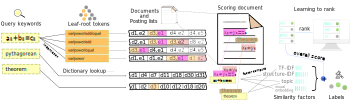
\includegraphics[width=1.0\textwidth]{img/architecture}
\caption{Overall architecture}
\end{figure*}
%%%%%%%%%%%%%%%%%%%%%%%%%%%%
\begin{figure*}[b!]
\centering
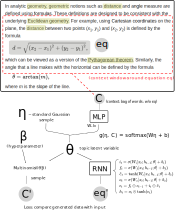
\includegraphics[width=0.6\textwidth]{img/lang-topic}
\caption{Topic-language model}
\end{figure*}

%%%%%%%%%%%%%%%%%%%%%%%%%%%%%%%%%%%%%%%%%%%%%%%%%%%%%%
\section{Design of Experiments}



\begin{table}

	\raggedright



    \caption{Experiments 1}

    \begin{tabular}{c|c}

		\hline

		design goal & Evaluate formula search effectiveness using IDF \\

		\hline

		dataset & Wiki-browsing, ARQMath task2  \\

	    \hline

		variables & number of subtrees to be measured, with or without IDF \\

		\hline

		metrics & Bpref, condensed and upperbound presion \\

		\hline

		compared systems & baseline of ECIR19, MCAT, Tangent-S

	\end{tabular}



	\vspace{1cm}

    \caption{Experiments 2}

    \begin{tabular}{c|c}

		\hline

		design goal & Evaluate formula search dynamic pruning efficiency on different thresholds \\

		\hline

		dataset & Wiki-browsing \\

	    \hline

		variables & threshold value, from 0\% to 50\% of the size of query expression \\

		\hline

		metrics & query run times, fully/partial Bpref scores, case studies \\

		\hline

		compared systems & baseline of ECIR19 \\

		\hline

		other notes & Show their query size differences \\

	\end{tabular}



	\vspace{1cm}

	\caption{Experiments 3}

	\begin{tabular}{c|c}

		\hline

		design goal & Given 1 second retrieval constraint, show the accuracy gain from adjusting parameters \\

		\hline

		dataset & MSE, ARQMath task2 \\

	    \hline

		variables & threshold value, number of trees to be matched, corpus size \\

		\hline

		metrics & query run times, fully/partial Bpref scores \\

		\hline

		compared systems & - \\

		\hline

		other notes & Achieving less than 1 second is required by user study~\cite{brutlag2008user} \\

	\end{tabular}



	\vspace{1cm}

	\caption{Experiments 4}

	\begin{tabular}{c|c}

		\hline

		design goal & investigate good embedding methods for visual appearance of formulas \\

		\hline

		dataset & Wiki-formula browsing \\

	    \hline

		variables & methods chosen from: fasttext, Dice, CBOW, ELMO, GloVe, RNN w/ attention, \\

		          & image2markup models. Different similarity measurement for embedding pairs \\

		\hline

		metrics & give a list of most similar formulas, case study. \\

		\hline

		compared systems & compare with \cite{BehroozICTIR2019} \\

	\end{tabular}



\end{table}



\begin{table}

    %\centering
	\raggedright



    \caption{Experiments 5}

	\begin{tabular}{c|c}

		\hline

		design goal & evaluate topic-language model effectiveness \\

		\hline

		dataset & MSE  \\

	    \hline

		variables & RNN units, neural network parameters, window size \\

		\hline

		metrics & cluster words and formulas by topics \\

		\hline

		compared systems & compare with Yale's topic-Eq and Blei math-embedding, \\

		& also compared with plain LDA, pLSA model. \\

	\end{tabular}



	\vspace{1cm}

	\caption{Experiments 6}

	\begin{tabular}{c|c}

		\hline

		design goal & text and formula mixed-search \\

		\hline

		dataset & NTCIR Wiki main corpus, ARQMath task2 \\

	    \hline

		variables & resemble models (structure search, visual embedding etc.), learning to rank methods \\

		\hline

		metrics & Bpref, condensed and upperbound  precision \\

		\hline

		compared systems & NTCIR participant systems \\

	\end{tabular}



\end{table}



%%%%%%%%%%%%%%%%%%%%%%%%%%%%



\section{Methodology}

\begin{itemize}

\item Structural search, single formula retrieval: Multi-tree search model

    \begin{itemize}

    \item scoring formulas

    \item algorithm to match operands/operators

    \end{itemize}

\item Dynamic pruning

    \begin{itemize}

    \item pruning threshold for formula

    \item GBP-NUM, GBP-LEN and MaxRef. Also a greedy binary programming solver.

    \end{itemize}

\item IDF weighting for formula token paths, probability model point of view.

    \begin{itemize}

    \item Scoring

    \item Index implementation + Pseudo code for traversing abstraction layer of hierarchical secondary inverted index.

    \end{itemize}

\item Embedding for math content (or text)

    \begin{itemize}

    \item FastText, Dice, CBOW, ELMO, Glove. Applying onto formula token paths.
	Because the space of formula leaf-root paths are huge, we may choose to only input a prefix sequence from leaf-root paths with limited prefix length.

    \item Visual embedding: A DenseNet image2markup model~\cite{zhang2017watch, yasunaga2019topiceq} (formula only). DenseNet is proposed on CVPR 2017, it provides shortcut links between every layer, while maintains relatively small number of parameters due to applying filters (in dense blocks) and pooling (in transition layers).
Unlike ResNet, DenseNet uses concatenation instead of addition when joining connections (see below), that means it has less correlated but more direct and diverse features feed to next layers, because addition creates dependency and add correlations between future outputs.
Also, DenseNet outputs k channels after each block, and does not change the size after each block. This makes it easy to stack the network blocks.

	\item Recent state-of-the-art model \textit{Multi-modal Attention Network} (MAN) ~\cite{wang2019multi} handles online HMER using attention mechanism, it employs DenseNet~\cite{huang2017densely} for offline image processing which converts image of pixels to annotation features $B$, it also uses bidirectional RNN to process online trajectory sequences and generate sequence feature $A$. 
The two latent features are then transformed into fixed-size context vector $c_t$ using multi-modal attention,
$$
c_t = f_{\mathrm{att}}(\hat h, A, B)
$$
where $\hat h$ is the RNN hidden state obtained from label sliding. Later, this multi-modal context is used to generate higher level sequence hidden state $h$, and output prediction is just a function of different level sequences we obtain:
$$
p(y_t|y_1 ... y_{t-1}, X) = \mathrm{softmax}(W_0 \cdot \phi(E y_{t-1} + W_h h_t + W_c c_t))
$$
However, because in Mathematics Information Retrieval (MIR), it is impractical to obtain trajectory information because index has to be built offline and from static document, we only take offline channel from MAN.
The offline channel attention uses sequence hidden state $\hat h_t$ from label as key, annotation features as query and coverage vectors $F = \{\hat f_i\}$ which accumulate past attentions:
$$
\begin{aligned}
\alpha_{ti} &= \mathrm{softmax}(v_{att}^T \; \mathrm{tanh} (W_{att} \hat{h}_t + U_{att} b_i + U_{f} \hat f_i)) \\
\hat F &= Q * \sum^{t-1}_l \alpha_{l}
\end{aligned}
$$
and the attention in offline channel is simply applied onto annotation features:
$$
\begin{aligned}
\hat c_t &= \sum_{i} \alpha_{ti} b_i \\
c_t &= \mathrm{tanh} (W_{fc} \; \hat c_t)
\end{aligned}
$$
this is the key difference compared to their previous work~\cite{zhang2017gru}, where online and offline information are considered as complementary information that determine final context together.


    \end{itemize}

\item Topic-language model to infer topic space

    \begin{itemize}

    \item Topic-Eq model with possibly some minor improvements.

    \item comparison to traditional pLSA, LDA models.

    \item RNN units

    \item variational neural network.

    \end{itemize}

\item Learning-to-rank methods

    \begin{itemize}

    \item RankNet, LambdaRank, LambdaMART and RankSVM reivew.

    \item formula and text features to be applied to learning-to-rank.

    \end{itemize}

\end{itemize}


\bibliographystyle{abbrv}
\bibliography{preproposal}

\section{Schedule (based on month, reformatted, still planing)}

\begin{table}[!b]
\newcommand*{\D}{\cellcolor{gray}}

\begin{center}
\resizebox{\linewidth}{!}{
\begin{tabular}{l| llllll | llll | llll | llll}

\multicolumn{1}{r}{}
& \multicolumn{6}{c}{Preparation}
& \multicolumn{4}{c}{Implementation}
& \multicolumn{4}{c}{Experiment}
& \multicolumn{4}{c}{Writeup}
\\ \hline

Month & 1 & 2 & 3 & 4 & 5 & 6 & 7 & 8 & 9 & 10 & 11 & 12 & 13 & 14 & 15 & 16 & 17 & 18
\\ \hline
\textbf{Method and Implementation}  & \\
\textbf{(i). formula search}          & \\

{\quad}One-tree formula w/ IDF and pruning &  &\D&\D&\D&\D&\D               \\
{\quad}Multi-tree formula w/ IDF           &  &\D&\D&\D&\D&\D               \\

\textbf{(ii). learning to rank}     & \\

{\quad}RankNet, LambdaRank, LambdaMART     &  &\D&\D&\D&\D&\D               \\
{\quad}Ranking SVM, IR SVM                 &  &\D&\D&\D&\D&\D               \\

\textbf{(iii). embedding / topic}   & \\

{\quad}LSTM, GRU language model            &  &  &  &  &  &  &  &  &\D&\D&\D \\
{\quad}DenseNet and visual embedding (WAP) &  &  &  &  &  &  &  &  &\D&\D&\D \\
{\quad}pLSA and LDA topic model            &  &  &  &  &  &  &  &  &\D&\D&\D \\
{\quad}VAE-based topic-language model      &  &  &  &  &  &  &  &  &  &  &\D&\D&\D  \\

\textbf{Evaluation / Experiments} & \\

{\quad}IDF-version formula search          &\D&\D&\D&\D&               \\
{\quad}Initial thresholds on efficiency    &  &  &  &\D&\D&            \\
{\quad}Mixed query (wiki-main)             &  &  &  &  &  &\D&  &  &\D&\D&\D&\D               \\

\textbf{Writing} & \\
{\quad}Introduction                        &  &  &  &  &  &  &  &  &  &  &\D&  &          \\
{\quad}Related work                        &  &\D&  &  &  &\D&  &  &  &\D&  &  &\D&    \\
{\quad}Methodology                         &  &  &  &  &  &  &  &  &\D&\D&\D&\D&  &\D      \\
{\quad}Experiments                         &  &  &\D&\D&\D&\D&  &  &  &  &  &  &\D&\D     \\
{\quad}Conclusion                          &  &  &  &  &  &  &  &  &  &  &  &  &  &\D       \\
\end{tabular}}
\end{center}

\caption{Timeline Table for Thesis Plan}
\end{table}

\end{document}
